% GNUPLOT: LaTeX picture with Postscript
\begingroup
  \makeatletter
  \providecommand\color[2][]{%
    \GenericError{(gnuplot) \space\space\space\@spaces}{%
      Package color not loaded in conjunction with
      terminal option `colourtext'%
    }{See the gnuplot documentation for explanation.%
    }{Either use 'blacktext' in gnuplot or load the package
      color.sty in LaTeX.}%
    \renewcommand\color[2][]{}%
  }%
  \providecommand\includegraphics[2][]{%
    \GenericError{(gnuplot) \space\space\space\@spaces}{%
      Package graphicx or graphics not loaded%
    }{See the gnuplot documentation for explanation.%
    }{The gnuplot epslatex terminal needs graphicx.sty or graphics.sty.}%
    \renewcommand\includegraphics[2][]{}%
  }%
  \providecommand\rotatebox[2]{#2}%
  \@ifundefined{ifGPcolor}{%
    \newif\ifGPcolor
    \GPcolortrue
  }{}%
  \@ifundefined{ifGPblacktext}{%
    \newif\ifGPblacktext
    \GPblacktexttrue
  }{}%
  % define a \g@addto@macro without @ in the name:
  \let\gplgaddtomacro\g@addto@macro
  % define empty templates for all commands taking text:
  \gdef\gplbacktext{}%
  \gdef\gplfronttext{}%
  \makeatother
  \ifGPblacktext
    % no textcolor at all
    \def\colorrgb#1{}%
    \def\colorgray#1{}%
  \else
    % gray or color?
    \ifGPcolor
      \def\colorrgb#1{\color[rgb]{#1}}%
      \def\colorgray#1{\color[gray]{#1}}%
      \expandafter\def\csname LTw\endcsname{\color{white}}%
      \expandafter\def\csname LTb\endcsname{\color{black}}%
      \expandafter\def\csname LTa\endcsname{\color{black}}%
      \expandafter\def\csname LT0\endcsname{\color[rgb]{1,0,0}}%
      \expandafter\def\csname LT1\endcsname{\color[rgb]{0,1,0}}%
      \expandafter\def\csname LT2\endcsname{\color[rgb]{0,0,1}}%
      \expandafter\def\csname LT3\endcsname{\color[rgb]{1,0,1}}%
      \expandafter\def\csname LT4\endcsname{\color[rgb]{0,1,1}}%
      \expandafter\def\csname LT5\endcsname{\color[rgb]{1,1,0}}%
      \expandafter\def\csname LT6\endcsname{\color[rgb]{0,0,0}}%
      \expandafter\def\csname LT7\endcsname{\color[rgb]{1,0.3,0}}%
      \expandafter\def\csname LT8\endcsname{\color[rgb]{0.5,0.5,0.5}}%
    \else
      % gray
      \def\colorrgb#1{\color{black}}%
      \def\colorgray#1{\color[gray]{#1}}%
      \expandafter\def\csname LTw\endcsname{\color{white}}%
      \expandafter\def\csname LTb\endcsname{\color{black}}%
      \expandafter\def\csname LTa\endcsname{\color{black}}%
      \expandafter\def\csname LT0\endcsname{\color{black}}%
      \expandafter\def\csname LT1\endcsname{\color{black}}%
      \expandafter\def\csname LT2\endcsname{\color{black}}%
      \expandafter\def\csname LT3\endcsname{\color{black}}%
      \expandafter\def\csname LT4\endcsname{\color{black}}%
      \expandafter\def\csname LT5\endcsname{\color{black}}%
      \expandafter\def\csname LT6\endcsname{\color{black}}%
      \expandafter\def\csname LT7\endcsname{\color{black}}%
      \expandafter\def\csname LT8\endcsname{\color{black}}%
    \fi
  \fi
    \setlength{\unitlength}{0.0500bp}%
    \ifx\gptboxheight\undefined%
      \newlength{\gptboxheight}%
      \newlength{\gptboxwidth}%
      \newsavebox{\gptboxtext}%
    \fi%
    \setlength{\fboxrule}{0.5pt}%
    \setlength{\fboxsep}{1pt}%
    \definecolor{tbcol}{rgb}{1,1,1}%
\begin{picture}(7360.00,2540.00)%
    \gplgaddtomacro\gplbacktext{%
      \csname LTb\endcsname%%
      \put(782,453){\makebox(0,0)[r]{\strut{}-2.0}}%
      \csname LTb\endcsname%%
      \put(782,798){\makebox(0,0)[r]{\strut{}-1.9}}%
      \csname LTb\endcsname%%
      \put(782,1142){\makebox(0,0)[r]{\strut{}-1.8}}%
      \csname LTb\endcsname%%
      \put(782,1486){\makebox(0,0)[r]{\strut{}-1.7}}%
      \csname LTb\endcsname%%
      \put(782,1831){\makebox(0,0)[r]{\strut{}-1.6}}%
      \csname LTb\endcsname%%
      \put(782,2175){\makebox(0,0)[r]{\strut{}-1.5}}%
      \csname LTb\endcsname%%
      \put(782,2519){\makebox(0,0)[r]{\strut{}-1.4}}%
      \csname LTb\endcsname%%
      \put(1114,277){\makebox(0,0){\strut{}$5$}}%
      \csname LTb\endcsname%%
      \put(1699,277){\makebox(0,0){\strut{}$10$}}%
      \csname LTb\endcsname%%
      \put(2283,277){\makebox(0,0){\strut{}$15$}}%
      \csname LTb\endcsname%%
      \put(2868,277){\makebox(0,0){\strut{}$20$}}%
      \csname LTb\endcsname%%
      \put(3452,277){\makebox(0,0){\strut{}$25$}}%
      \csname LTb\endcsname%%
      \put(4036,277){\makebox(0,0){\strut{}$30$}}%
      \csname LTb\endcsname%%
      \put(2458,660){\makebox(0,0){\strut{}VBS Antiparallel}}%
    }%
    \gplgaddtomacro\gplfronttext{%
      \csname LTb\endcsname%%
      \put(229,1486){\rotatebox{-270.00}{\makebox(0,0){\strut{}Energy (eV)}}}%
      \csname LTb\endcsname%%
      \put(2458,13){\makebox(0,0){\strut{}Distance (\AA)}}%
    }%
    \gplgaddtomacro\gplbacktext{%
      \csname LTb\endcsname%%
      \put(4085,453){\makebox(0,0)[r]{\strut{}}}%
      \csname LTb\endcsname%%
      \put(4085,798){\makebox(0,0)[r]{\strut{}}}%
      \csname LTb\endcsname%%
      \put(4085,1142){\makebox(0,0)[r]{\strut{}}}%
      \csname LTb\endcsname%%
      \put(4085,1486){\makebox(0,0)[r]{\strut{}}}%
      \csname LTb\endcsname%%
      \put(4085,1831){\makebox(0,0)[r]{\strut{}}}%
      \csname LTb\endcsname%%
      \put(4085,2175){\makebox(0,0)[r]{\strut{}}}%
      \csname LTb\endcsname%%
      \put(4085,2519){\makebox(0,0)[r]{\strut{}}}%
      \csname LTb\endcsname%%
      \put(4417,277){\makebox(0,0){\strut{}$5$}}%
      \csname LTb\endcsname%%
      \put(5002,277){\makebox(0,0){\strut{}$10$}}%
      \csname LTb\endcsname%%
      \put(5586,277){\makebox(0,0){\strut{}$15$}}%
      \csname LTb\endcsname%%
      \put(6171,277){\makebox(0,0){\strut{}$20$}}%
      \csname LTb\endcsname%%
      \put(6755,277){\makebox(0,0){\strut{}$25$}}%
      \csname LTb\endcsname%%
      \put(7339,277){\makebox(0,0){\strut{}$30$}}%
      \csname LTb\endcsname%%
      \put(5761,660){\makebox(0,0){\strut{}VBS Parallel}}%
    }%
    \gplgaddtomacro\gplfronttext{%
      \csname LTb\endcsname%%
      \put(6584,2361){\makebox(0,0)[r]{\strut{}$\mathrm{CH}_4$}}%
      \csname LTb\endcsname%%
      \put(6584,2185){\makebox(0,0)[r]{\strut{}$\mathrm{NH}_3$}}%
      \csname LTb\endcsname%%
      \put(6584,2009){\makebox(0,0)[r]{\strut{}$\mathrm{H}_2\mathrm{O}$}}%
      \csname LTb\endcsname%%
      \put(6584,1833){\makebox(0,0)[r]{\strut{}$\mathrm{HF}$}}%
      \csname LTb\endcsname%%
      \put(5761,13){\makebox(0,0){\strut{}Distance (\AA)}}%
    }%
    \gplbacktext
    \put(0,0){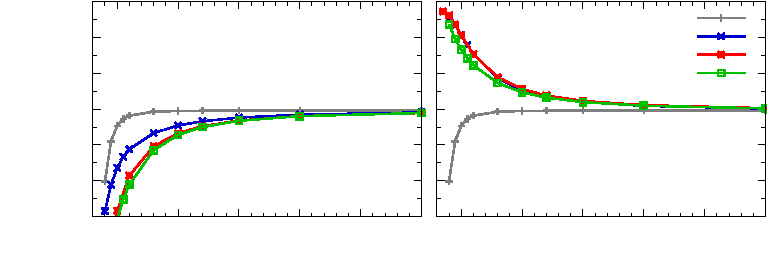
\includegraphics[width={368.00bp},height={127.00bp}]{Figs/scan_VBS}}%
    \gplfronttext
  \end{picture}%
\endgroup
